\documentclass[11pt,a4paper,oneside]{article}
\usepackage{parskip}
\usepackage{graphicx}
\usepackage{url}
\graphicspath{ {./images/} }

\title{CQS: Command Query Separation}
\author{Andreas Wenzelhuemer}

\begin{document}

\maketitle

The topic of this pattern will be about the architectural pattern called Command Query Separation~\footnote{\url{https://martinfowler.com/bliki/CQRS.html}}.
CQS is a principle or a guideline, that states that every method should be a command or a query (see figure~\ref{fig:cqs}).

\begin{figure}[h]
    \centering
    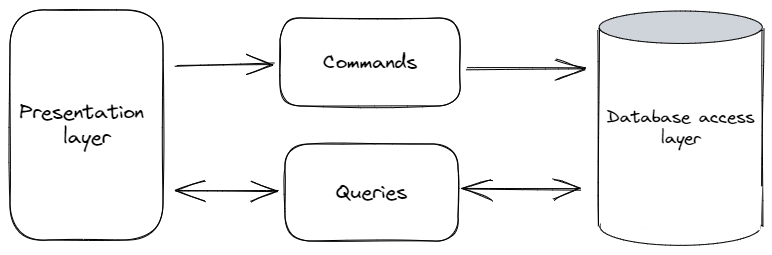
\includegraphics[width=0.65\textwidth]{images/CQS.png}
    \caption{CQS}
    \label{fig:cqs}
\end{figure}

\begin{itemize}
    \item {Query: Is responsible for returning the correct values without modifying anything (There are no side effects).}
    \item {Command: Changes the state of the system but does not return any values.}
\end{itemize}

There exist multiple different implementations, but normally there is one object for representing the operation and a handler class, which contains the actual implementation.
A so called dispatcher object is responsible for passing the given request to the correct handler.
Additionally here is also an extension of the pattern, the so called Command Query Responsibility Segregation (CQRS).
The difference in contrast to CQS is, that updates and reads are performed on separate databases and the read database gets synchronized when the data in the other database gets updated.

So the paper will contain the following topics:
\begin{itemize}
    \item {CQS: What is it and how to use it.}
    \item {CQRS: What is the difference between CQS and CQRS.}
    \item {Code examples from a small prototype written in C\#}
\end{itemize}

\end{document}
